\documentclass{beamer}
\usepackage{booktabs}
\usepackage{graphicx}
\usepackage{amsmath}
\usepackage{array}
\usepackage{multirow}
\usetheme{default}
\setbeamertemplate{navigation symbols}{}
\setbeamertemplate{footline}{\hfill\insertframenumber/\inserttotalframenumber\hspace{1.5em}}

\title{Robust Constraint Learning: Research Update}
\subtitle{The shared-$D$ $\rho$ sweep; a conformal competitor}
\date{19 August 2026}

\begin{document}

\begin{frame}
  \titlepage
  \begin{center}\footnotesize
  Supersedes the 10 Aug deck. Standing method reference: \texttt{method.tex}.
  \end{center}
\end{frame}

% ===========================================================================
\begin{frame}{Summary}
  \small
  \begin{itemize}
    \item \textbf{One shared ellipsoidal $D$, swept on $\rho$.}
    \item \textbf{CP is the only method to clear feasibility $0.9$ throughout}
      --- gastric all 7 $\rho$; synthetic the only method to reach it at all.
    \item \textbf{Robustness is cheap early, dear late.} Gastric CP: $+5.5$ pts
      feasibility for $-0.23$ months OS at $\rho{=}0.1$; the next $+0.8$ pts
      costs $-1.16$ months.
    \item \textbf{Tradeoffs between feasibility, objective, solvability, speed}.
    \item \textbf{The fixed dials were not cherry-picked.} $\tau$ saturates;
      $\alpha$ is a genuine frontier.
    \item \textbf{Next:} select $\rho^*$, confirm $\rho^*$ on the \emph{test} set under
      m-out-of-n; C-MICL as a fifth method.
  \end{itemize}
\end{frame}

% ===========================================================================
\begin{frame}{The $\rho$ sweep --- protocol}
  \small
  One shared $D$ per outcome $c$; every method faces it at each $\rho$.
  \vspace{-0.4em}
  \[
    D_c=\{\delta\in\mathbb{R}^{n}:\|\delta\|_2\le R_c\},\quad
    R_c=\rho\,\mathrm{scale}(y_c)\sqrt{n}
  \]
  \vspace{-1.2em}
  \begin{itemize}
    \item $\mathrm{scale}(y_c)$ = out-of-fold residual sd. $\delta$ added to
      $y_c$ \emph{before} training; model refit.
    \item Grid $\rho\in\{0.05,0.1,0.2,0.3,0.5,0.75,1\}$. $\rho{=}1$ = iid noise
      at one unexplained sd per row.
    \item Own dials \emph{fixed}: CP $\tau{=}0.01$, wrapper $\alpha{=}0.2$.
      Ablated separately at $\rho{=}1$.
    \item Scored on CV folds of \emph{train} (4 temporal / 4 KFold). The real
      test set is not used here.
    \item \textbf{$\rho^*$ rule (derived, not fitted):} largest grid $\rho$ with
      held-out feasibility $\ge0.9$ \emph{and} solved fraction $\ge0.5$.
  \end{itemize}
\end{frame}

% ===========================================================================
\begin{frame}{Feasibility vs $\rho$}
  \begin{center}
  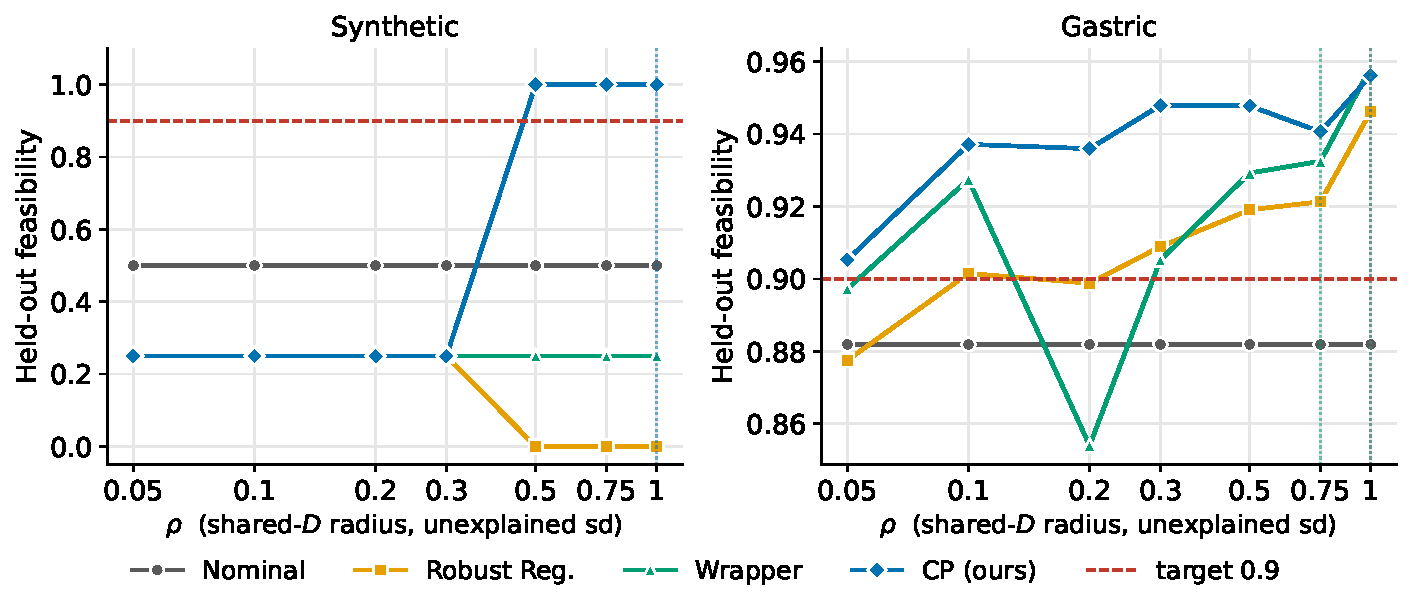
\includegraphics[width=\linewidth]{../results/figures/fig_rho_feasibility.pdf}
  \end{center}
  \vspace{-0.3em}
  {\footnotesize
  Note the panels' $y$-scales differ. Dotted verticals = $\rho^*$ --- gastric CP
  and robust\_reg both $1.0$ (coincident), wrapper $0.75$; synthetic CP only.
  Synthetic feasibility resolves only to $0.25$ (4 folds).}
\end{frame}

\begin{frame}{Feasibility --- what it says}
  \small
  \begin{itemize}
    \item \textbf{Gastric: CP clears $0.9$ at all 7 $\rho$.} Wrapper 5/7,
      robust\_reg 5/7, nominal 0/7 (flat $0.882$).
    \item CP $0.905\!\to\!0.956$ across the axis; $+5.5$ pts over nominal
      already at $\rho{=}0.1$.
    \item Wrapper is non-monotone --- $0.927$ at $\rho{=}0.1$, $0.854$ at
      $\rho{=}0.2$. Random draws, $P{=}20$.
    \item \textbf{Synthetic: only CP ever reaches the target}, and only at
      $\rho\ge0.5$ ($1.00$). Nominal $0.50$, wrapper $0.25$ throughout.
    \item robust\_reg on synthetic \emph{falls} to $0.0$ for $\rho\ge0.5$. See
      the objective slide --- wrong direction.
  \end{itemize}
\end{frame}

% ===========================================================================
\begin{frame}{Objective vs $\rho$ --- the price}
  \begin{center}
  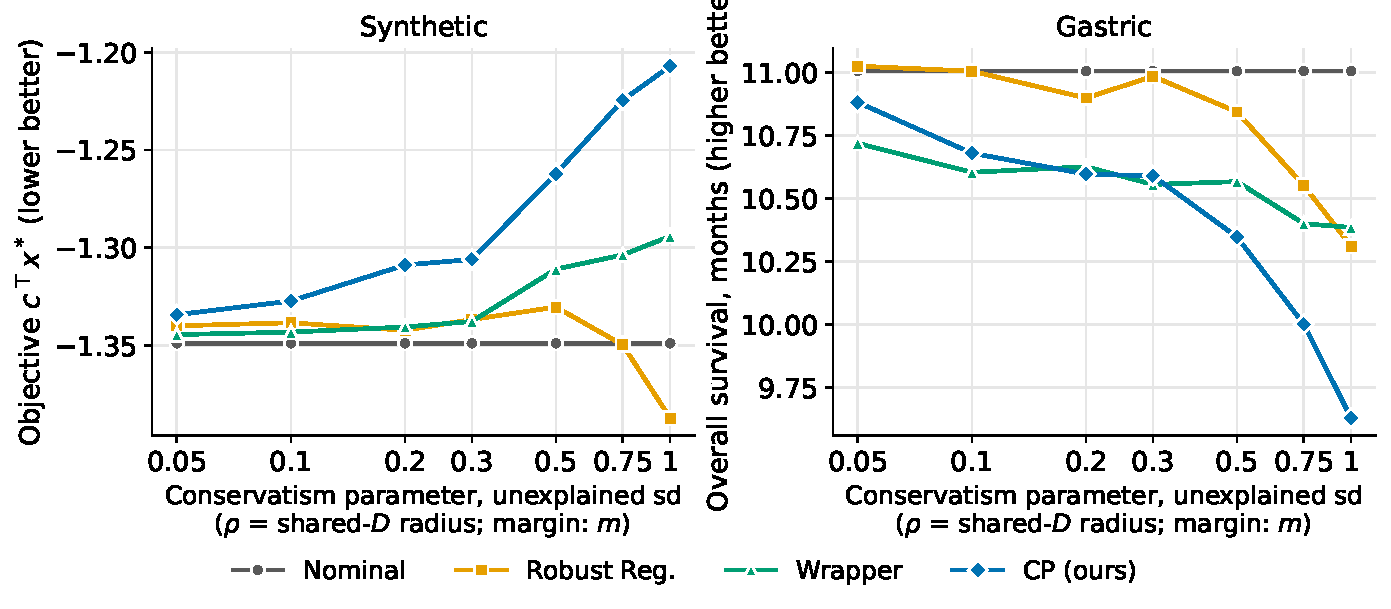
\includegraphics[width=\linewidth]{../results/figures/fig_rho_objective.pdf}
  \end{center}
  \vspace{-0.3em}
  {\footnotesize Nominal ignores $\rho$, so its line is flat by construction.}
\end{frame}

\begin{frame}{Price --- what it says}
  \small
  \begin{itemize}
    \item \textbf{Robustness is cheap early.} Gastric CP at $\rho{=}0.1$:
      $+5.5$ pts feasibility for $-0.23$ months OS ($-2.0\%$).
    \item \textbf{Then it is not.} $\rho\,0.3\!\to\!1$ buys $+0.8$ pts
      ($0.948\!\to\!0.956$) for $-1.16$ months.
    \item Wrapper is flatter in cost but never gets above $0.958$ either.
    \item Synthetic CP: $+6.5\%$ objective at $\rho{=}0.5$, $+10.5\%$ at
      $\rho{=}1$, for $0.25\!\to\!1.00$ feasibility.
    \item \textbf{Anomaly.} Synthetic robust\_reg at $\rho{=}1$ scores
      $-1.387$ --- \emph{better} than nominal $-1.349$ --- at feasibility $0$.
      The shifted-label refit loosened the constraint. Not yet diagnosed.
  \end{itemize}
\end{frame}

% ===========================================================================
\begin{frame}{Solved fraction --- the artefact guard}
  \begin{center}
  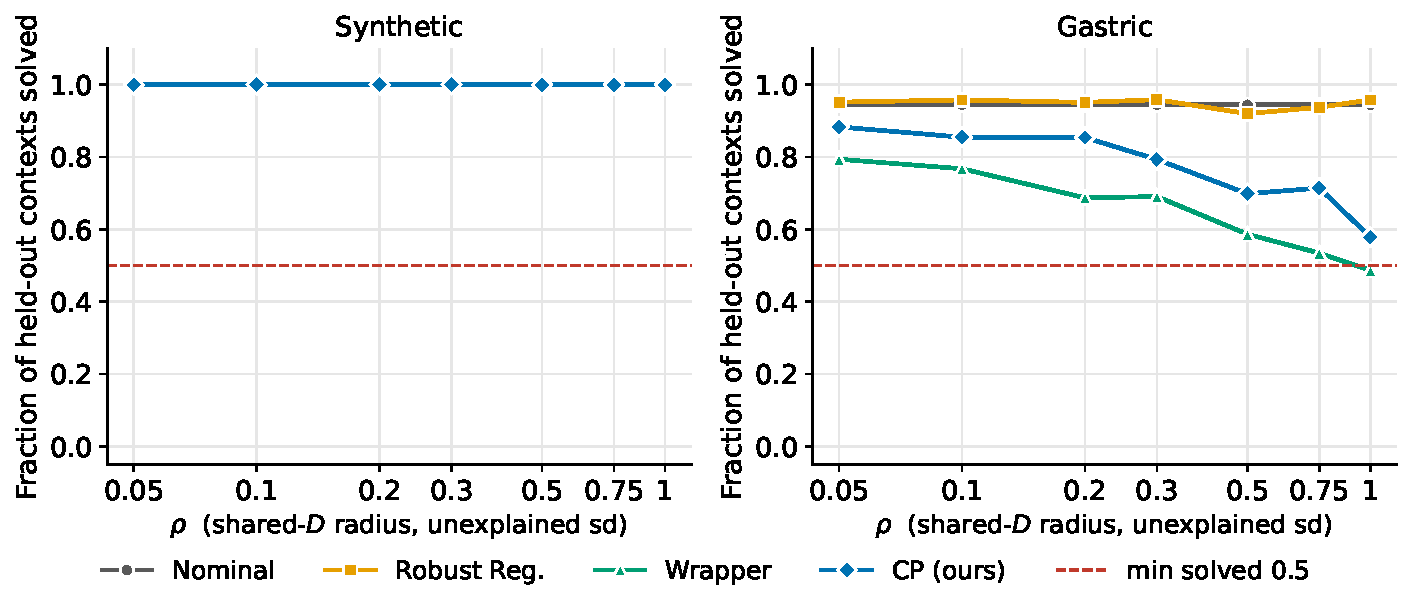
\includegraphics[width=\linewidth]{../results/figures/fig_rho_solved.pdf}
  \end{center}
  \vspace{-0.4em}
  {\footnotesize Yes --- every feasibility/objective number so far is conditional
  on the method returning a prescription, over its \emph{own} solved contexts.
  Hence this slide: high feasibility on few survivors is not a win. Floor $=0.5$.}
\end{frame}

\begin{frame}{Solved fraction --- what it says}
  \small
  \begin{itemize}
    \item \textbf{Gastric conservatism renders contexts unsolvable.} Wrapper
      $0.79\!\to\!0.49$, CP $0.88\!\to\!0.58$ over the axis.
    \item robust\_reg holds $0.92$--$0.96$ throughout: its adversary shapes the
      \emph{fit}, never becomes a constraint.
    \item Wrapper drops below the $0.5$ floor at $\rho{=}1$ ($0.487$) --- that
      cell is dropped from $\rho^*$.
    \item Synthetic: $1.0$ for every method at every $\rho$. Not contextual.
    \item \textbf{Every cell converged}: \texttt{n\_capped}${=}0$ throughout,
      no \texttt{max\_iterations}.
  \end{itemize}
\end{frame}

% ===========================================================================
\begin{frame}{$\rho^*$ --- derived, at feasibility $\ge0.9$, solved $\ge0.5$}
  \small
  \begin{center}
  \begin{tabular}{llccccc}
    \toprule
    & Method & $\rho^*$ & Feas. & Obj. & Solved & Master (s)\\
    \midrule
    \multirow{4}{*}{Gastric}
      & CP          & $1.0^\dagger$  & 0.956 & 9.45  & 0.58 & 651\\
      & robust\_reg & $1.0^\dagger$  & 0.946 & 10.53 & 0.96 & 1.9\\
      & wrapper     & $0.75^\ddagger$& 0.932 & 10.43 & 0.53 & 37\\
      & nominal     & ---            & \multicolumn{4}{l}{never reaches $0.9$}\\
    \midrule
    \multirow{2}{*}{Synth.}
      & CP          & $1.0^\dagger$  & 1.00  & $-1.207$ & 1.00 & 123\\
      & others      & ---            & \multicolumn{4}{l}{never reach $0.9$}\\
    \bottomrule
  \end{tabular}
  \end{center}
  \medskip
  {\footnotesize
  $\dagger$ censored: grid ran out, $\rho^*$ is a lower bound.\\
  $\ddagger$ \emph{not} grid-censored --- the wrapper's $\rho{=}1$ cell fell
  below the solved floor. CSV records this as \texttt{bound=solved\_floor}.}
\end{frame}

\begin{frame}{$\rho^*$ --- read it honestly}
  \small
  \begin{itemize}
    \item \textbf{CP and robust\_reg both censor at the grid max on gastric.}
      $\rho^*$ does not separate them; the curve and the cost do.
    \item robust\_reg is cheaper on every axis \emph{but the one that matters}
      --- $+1.08$ months OS, $+0.38$ solved, $340\times$ less master time, but
      $-1.0$ pt held-out feasibility ($0.946$ vs CP's $0.956$).
    \item \textbf{But its adversary is directed and CP's is random.} Same $D$,
      same budget, unequal strength (best-of-$B$ random ${\approx}64\%$ of
      directed on synthetic). Not a like-for-like win.
    \item $B{=}200$ vs $P{=}20$ confounds CP vs wrapper, but since we only add
      one at a time in CP, this is expected.
  \end{itemize}
\end{frame}

% ===========================================================================
\begin{frame}{Where the wall clock goes (gastric)}
  \begin{center}
  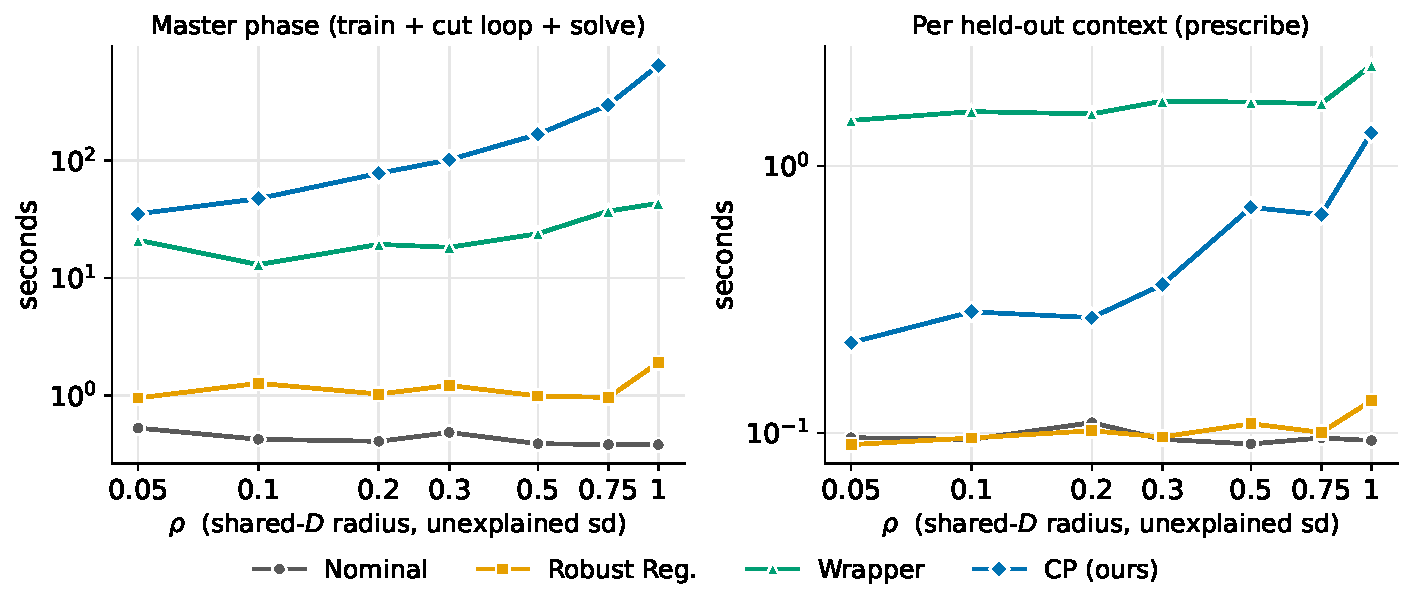
\includegraphics[width=\linewidth]{../results/figures/fig_rho_time.pdf}
  \end{center}
  \vspace{-0.4em}
  {\footnotesize Master = train + cut loop + final solve. Log scale.}
\end{frame}

\begin{frame}{Cost profile --- the MIP-size claim}
  \small
  \begin{itemize}
    \item \textbf{CP pays up front, wrapper pays per prescription.} At
      $\rho{=}0.1$: CP $47.5$s $+0.28$s/pt; wrapper $13.0$s $+1.60$s/pt.
    \item Crossover at ${\approx}26$ held-out contexts. CP prescribes
      $5.6\times$ faster.
    \item \textbf{The claim degrades with $\rho$.} At $\rho{=}1$: CP $651$s
      $+1.33$s/pt vs wrapper $43$s $+2.38$s/pt --- crossover ${\approx}580$
      contexts.
    \item CP master time grows $18\times$ over the axis; the cut loop, not the
      master solve.
    \item robust\_reg is ${\approx}1$--$2$s master and $0.1$s/pt at every
      $\rho$. It trains one model.
  \end{itemize}
\end{frame}

% ===========================================================================
\begin{frame}{Ablations at $\rho=1$ --- the dials were not cherry-picked}
  \begin{center}
  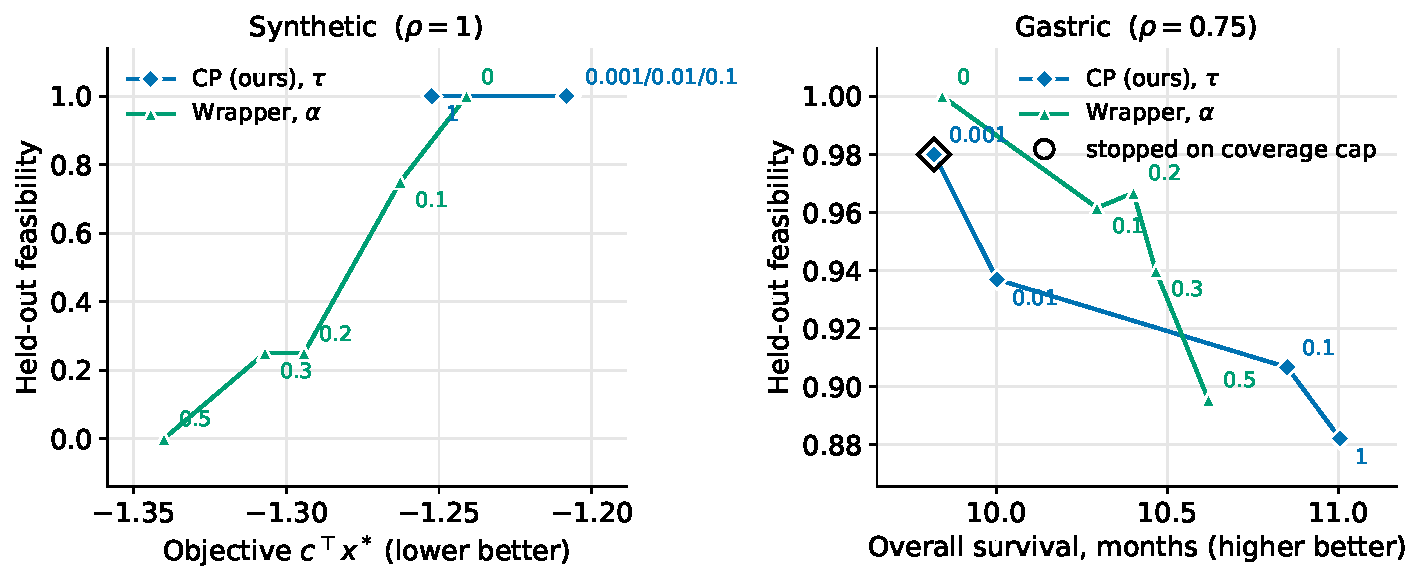
\includegraphics[width=\linewidth]{../results/figures/fig_rho_ablation.pdf}
  \end{center}
  \vspace{-0.4em}
  {\footnotesize Points labelled with the knob value; $\tau$ decreasing and
  $\alpha$ increasing are opposite directions of conservatism.}
\end{frame}

\begin{frame}{Ablations --- what they say}
  \small
  \begin{itemize}
    \item \textbf{$\tau$ saturates.} Gastric $0.01\!\to\!0.001$ moves nothing
      ($0.956\!\to\!0.950$ feas, OS $9.448\!\to\!9.452$); both stop on the
      coverage cap, not on $\tau$. Synthetic: $0.1/0.01/0.001$ coincide.
    \item So fixing $\tau{=}0.01$ costs nothing measurable --- and CV
      saturating at the strong end was the right read.
    \item \textbf{$\tau{=}1$ returns nominal exactly} on gastric
      ($11.005$, $0.882$). The decade grid does span nominal.
    \item \textbf{$\alpha$ is a genuine frontier.} Gastric $0\!\to\!0.5$:
      feas $1.00\!\to\!0.84$, OS $9.67\!\to\!10.60$, monotone.
    \item \textbf{But $\alpha{=}0$ solves only $0.32$ of contexts.} Its
      feasibility $1.00$ is the survivor artefact, not a result.
  \end{itemize}
\end{frame}

% ===========================================================================
\begin{frame}{Next: confirm $\rho^*$ on the test set}
  \small
  \textbf{Rerun the m-out-of-n probe at \texttt{geometry: ellipsoid}.}
  $R$ training subsamples, without replacement; prescribe over the real
  \texttt{X\_test}; score against the GT ensemble fit on the full clean cohort.
  \begin{itemize}
    \item \textbf{Why.} The sweep varies CV folds of \emph{train} only, on one
      training draw --- $\rho^*$ carries no training-draw error bars. CP $0.956$
      vs robust\_reg $0.946$ is 1 pt on 4 folds.
    \item \textbf{Not in the sweep itself.} $\rho^*$ is read off that curve;
      scoring it on test spends the test set on a tuning decision.
    \item \textbf{One shared $\rho$, not $\rho^*(\text{method})$.} $\rho{=}0.75$
      --- largest where all three clear feasibility $0.9$ \emph{and} the solved
      floor. $\rho{=}1$ as a stress cell.
    \item \textbf{All current Table 6 numbers predate $\rho$}
      (\texttt{box\_l1}, $\varepsilon_0{=}1$), so nothing is at $\rho^*$ yet.
  \end{itemize}
\end{frame}

% ===========================================================================
\begin{frame}{Open after this sweep}
  \small
  \begin{itemize}
    \item \textbf{Diagnose synthetic robust\_reg at $\rho\ge0.5$}: objective
      better than nominal, feasibility $0$.
    \item \textbf{Extend the grid past $\rho{=}1$} --- two of three gastric
      $\rho^*$ are censored, so the axis has not been resolved.
    \item \textbf{Settled: the adversary asymmetry stays.} Directed cuts in
      CP/wrapper accumulate until the master admits nothing --- infeasibility
      too high. Report the ${\approx}64\%$ gap; do not equalise.
  \end{itemize}
\end{frame}

% ===========================================================================
\begin{frame}{C-MICL --- conformal, not ensemble}
  Ovalle et al.\ 2025, arXiv 2506.03531. Wrapper's target, different mechanism.
  \begin{enumerate}
    \item Fit $\hat h$ (80\%); fit $\hat u$ on $|\hat h(x)-y|$.
    \item Calibrate (20\%, $N$): $\hat q$ = quantile of $|\hat h-y|/\hat u$ at
      $(1-\alpha)(1+1/N)$.
    \item Embed $\hat h\pm\hat q\,\hat u\subseteq[\underline y,\overline y]$ ---
      two linear constraints.
  \end{enumerate}
  \medskip
  \begin{itemize}
    \item Two models, not $P$. Size independent of $N$.
    \item $\ge0.90$ coverage on every base model.
    \item ${\approx}8\%$ objective; $10^2\times$ faster than W-MICL(50).
  \end{itemize}
\end{frame}

% ===========================================================================
\begin{frame}{Limitations}
  \small
  \begin{itemize}
    \item \textbf{Assumption 4.1 carries it.}
      $\mathcal F_N=\{\mathcal C(x)\subseteq\mathcal Y\}$ passes where $\hat u$ is
      small --- where the model claims confidence. Overconfidence is
      over-represented among the feasible. Assumed, not derived.
    \item \textbf{Exchangeability.} Gastric splits on publication year. Random
      calibration split leaks; temporal one voids the guarantee.
    \item \textbf{Does not extend.} Marginal coverage \emph{per outcome}, not
      joint over 5. Their $x$ = all decisions; ours conditions on $z$ ---
      conditional coverage, distribution-free impossible (ref.\ 44).
    \item \textbf{No frontier.} Two $\alpha$ points; W-MICL swept on $P$, not
      $\alpha$. Maragno Fig.\ 7: $\alpha{=}0$ vs $0.5$ $=+11.3\%$ palatability
      for $+2.5\%$ cost.
  \end{itemize}
\end{frame}

% ===========================================================================
\begin{frame}{Next: C-MICL as a fifth method}
  \small
  \textbf{Expect infeasible on gastric --- that is the result.}
  \begin{itemize}
    \item Unexplained $0.78$--$1.02$ $\Rightarrow$ $\hat u\approx\mathrm{sd}(y)$
      $\Rightarrow$ ${\approx}1.65\,\mathrm{sd}(y)$ half-width $\times$ 5
      constraints.
    \item Their own stated limitation: poor $\hat h$ $\Rightarrow$ sets too wide
      $\Rightarrow$ infeasible.
    \item CP absorbs the same fit by \emph{cutting the worst scenario}, not
      inflating uniformly.
  \end{itemize}
  \medskip
  \textbf{Decisions first}
  \begin{itemize}
    \item Joint coverage: max-over-outcomes ($N\ge9$) vs Bonferroni $\alpha/6$
      ($N\ge59$; 64 arms $\Rightarrow$ $\hat q$ = sample max).
    \item Context: Mondrian strata, or marginal-only and say so.
    \item Calibration split vs.\ the temporal protocol.
  \end{itemize}
\end{frame}

\end{document}
